\chapter{불덩이, 기준계, 그리고 4-벡터}

고에너지 충돌을 논의하다 남겨 둔 질문부터 시작하자. 무거운 원자핵 두 개의 충돌은 조용한 천체 블랙홀이 아니라 격렬하게 변하는 물체를 만들어 낸다. 그렇다면 그 충돌을 지평선으로 기술한다는 것은 무슨 뜻일까? 답을 찾아가려면 강하게 결합된 물질을 5차원으로 그린 그림, 가속기에 관한 실용적인 질문들, 그리고 마지막으로 특수 상대성 이론의 기하학으로 돌아가야 한다. 끝에 이르면 속도와 운동량은 4-벡터가 되고, 에너지는 운동량의 세 성분과 나란히 놓인다.

\section{5차원의 불덩이}

\begin{classroomqa}
\audiencequestion{충돌로 생긴 물체는 불안정하고 모양도 변합니다. 어떻게 이렇게 복잡한 물체를 블랙홀이라고 부를 수 있나요?}
\lecturerresponse{바닥과 천장 사이에 5번째 공간 방향이 뻗어 있다고 생각해 보자. 그 방향의 중력은 들뜸을 바닥 쪽으로 끌어당긴다. 충돌은 그곳에 뜨거운 에너지 덩어리를 남긴다. 덩어리는 퍼지고 모양도 바뀌지만, 지평선과 온도, 엔트로피를 가질 수 있다.}
\end{classroomqa}

이 5차원 세계에서 입자, 또는 그림을 좀 더 쉽게 떠올리자면 작은 끈들이 움직인다고 상상해 보자. 바닥으로 떨어지는 들뜸은 4차원에서 하드론, 즉 양성자, 중성자, 중간자와 그 밖의 크기를 가진 복합 물체로 나타난다. 천장 가까이에 붙어 있는 들뜸은 더 기본적인 입자처럼 보인다. 따라서 수직 방향의 위치는 규모를 부호화하는 기하학적 방식이다. 바닥은 장거리 하드론 영역을, 천장은 단거리 자유도를 나타낸다.

두 하드론이 충돌하면 바닥 가까이에 있던 두 물체가 서로 부딪치며 큰 에너지 물보라를 일으킨다. 그 결과는 강체가 아니다. 5차원 중력장에 놓인, 일종의 웅덩이 같은 뜨거운 덩어리이며 지평선을 지닌다. 이는 보통의 4차원 공간에 있는 천체 블랙홀도 아니고, 천장에 붙어 있는 플랑크 규모의 블랙홀도 아니다. 바닥 가까이에서 강하게 상호작용하는 불덩이를 중력으로 기술한 것이다.

고에너지에서 입사하는 원자핵은 로런츠 수축을 거쳐 얇은 팬케이크 모양이 된다. 이들은 충돌해 작은 영역에 에너지를 남기고, 평형을 향해 퍼져 나가는 유체를 만들어 낸다. 점성이 작다는 점은 쿼크--글루온 플라스마에서 놀라웠던 특징 가운데 하나였다. 5차원 기술에서 같은 진화는 일그러진 지평선이 이완되는 과정이다.

\begin{figure}[H]
\centering
\includegraphics[width=0.82\textwidth]{lecture_05_figure_01.png}
\caption{5차원 방향을 바닥과 천장으로 나타낸 그림. 가운데의 지평선을 지닌 덩어리는 충돌 뒤 바닥을 따라 퍼진다.}
\lectureframe{00:04:22}
\end{figure}

지평선이 영원히 남아 있지는 않는다. 호킹 복사가 에너지를 실어 나가며, 4차원 기술에서 그 복사는 충돌로부터 나오는 보통 하드론의 다발이다. 검출기 사건에서 관측되는 수천 개의 궤적은 이 표현으로 말하자면 쌍대 블랙홀에서 끓어 나와 방출된 입자들이다.

\subsection{추가 차원은 실재하는가?}

\begin{classroomqa}
\audiencequestion{5번째 차원은 공간 차원인가요? 바닥과 천장을 잇는 선은 실제로 그 방향으로 뻗어 있나요?}
\lecturerresponse{그렇다. 이는 공간꼴 차원이고, 5차원 기하학에서 그린 면은 지평선이다. 추가 방향을 ``실재''한다고 부를지, 아니면 동등한 수학적 기술로 볼지는 더 깊은 질문이다.}
\end{classroomqa}

유용한 설명은 중력이 양자 색역학을 대체한다는 것이 아니다. 오히려 두 가지 언어가 같은 물리를 기술할 수 있다. 4차원 언어에는 보통의 중력장이 없는 뜨거운 쿼크와 글루온의 불덩이가 있다. 5차원 언어에는 중력과 지평선이 있다. 대응 관계가 옳다면, 두 방식으로 모두 계산할 수 있는 영역에서는 엄밀한 QCD 계산과 쌍대 중력 계산이 일치해야 한다.

\begin{classroomqa}
\audiencequestion{QCD에는 중력도 지평선도 없습니다. 블랙홀 그림이 새로운 물리를 더하는 건가요, 아니면 불덩이를 다른 방식으로 기술할 뿐인가요?}
\lecturerresponse{4차원에서는 쿼크와 글루온의 플라스마이고, 5차원으로 구현하면 지평선을 가진 중력 기술이 있다. 이점은 계산에 있다. 강하게 결합된 QCD는 매우 어려운 반면, 지평선의 일부 성질---특히 점성---은 비교적 쉽게 계산할 수 있다.}
\end{classroomqa}

``실재하는 차원''과 ``수학적 유사성''의 구분을 확정해야만 이 기술을 유용하게 쓸 수 있는 것은 아니다. 어떤 구조가 다른 변수들을 더 단순하고 일관성 있는 법칙으로 묶어 준다면, 그 구조에는 물리적 해석을 부여할 만하다. 그래도 주장을 지나치게 확대해서는 안 된다. 관측된 쿼크--글루온 플라스마에 게이지/중력 쌍대성을 적용한 것은 강결합 동역학의 모형이지, 현실의 QCD에 알려진 정확한 중력 쌍대가 있다는 증명은 아니다.\editorialnote{이 단서는 QCD 응용의 현대적 지위를 명시한다. 여기서 전개한 5차원 메커니즘을 바꾸지는 않는다.}

\section{충돌형 가속기에서 빔을 충돌시키는 이유}

이제 질문은 실용적인 문제로 옮겨간다. 정지 표적에 단일 빔을 쏘는 대신 움직이는 빔 두 개를 쓰는 이유는 무엇일까? 원형 가속기는 왜 그렇게 클까? 전자와 양성자를 서로 다르게 다루는 이유는 무엇일까? 이 모든 질문은 상대론적 에너지에 관한 것이다.

\begin{classroomqa}
\audiencequestion{에너지가 큰 빔 하나를 정지 표적에 쏘는 대신 빔 두 개를 충돌시키는 이유는 무엇인가요?}
\lecturerresponse{새 입자를 만들어 내는 것은 질량중심계에서 이용할 수 있는 에너지다. 크기가 같고 서로 반대 방향으로 진행하는 상대론적 빔 두 개는 알짜 운동량이 없으므로, 에너지의 거의 전부를 충돌에 사용할 수 있다. 고정 표적을 쓰면 입사 에너지의 상당 부분이 질량중심 자체의 운동으로 남는다.}
\end{classroomqa}

크기가 \(p\)이고 서로 반대 방향으로 움직이는 두 초상대론적 입자에 대해, 강의 수준에서 \(c=1\) 단위로 어림하면
\begin{equation}
E_{\mathrm{cm}}^{\mathrm{collider}}\simeq 2p.
\end{equation}
이에 대응하는 고정 표적의 어림값은 빔 운동량의 제곱근에 비례해 증가할 뿐이다.
\begin{equation}
E_{\mathrm{cm}}^{\mathrm{fixed}}\sim \sqrt{mp}.
\end{equation}
생략한 수치 계수가 아니라 스케일링이 핵심이다. 빔 에너지를 두 배로 하면 충돌형 가속기의 질량중심 에너지도 두 배가 되지만, 고정 표적에서의 질량중심 에너지는 제곱근만큼만 증가한다.

불변량을 이용한 계산으로 두 경우를 정확히 비교할 수 있다. 입사하는 4-운동량이 \(P_1\)와 \(P_2\)라면,
\begin{equation}
s=(P_1+P_2)^2,
\qquad E_{\mathrm{cm}}=\sqrt{s}.
\end{equation}
에너지가 \(E\)인 동일한 역방향 빔에서는 공간 운동량이 상쇄되어 \(\sqrt{s}=2E\)가 된다. 정지해 있는 같은 질량의 표적에 에너지가 \(E\gg m\)인 발사체가 충돌하는 경우에는,
\begin{equation}
s=2m^2+2mE,
\qquad
\sqrt{s}\simeq \sqrt{2mE}
\qquad (c=1).
\end{equation}
이 짧은 불변량 유도로 앞서 말로 제시한 어림값에서 생략된 계수를 구할 수 있다.\editorialnote{이 유도를 넣어 강의의 스케일링 논증을 재현할 수 있게 했다.}

\begin{classroomqa}
\audiencequestion{원형 가속기가 반드시 그렇게 커야 하는 근본적인 이유가 있나요? 같은 빔을 더 작은 장치 안에서 여러 번 돌리면 안 되나요?}
\lecturerresponse{장과 재료가 한계를 정한다. 입자는 미터당 유한한 에너지만 얻으므로, 더 높은 에너지의 장치에는 더 긴 유효 가속 구간이 필요하다. 또한 원을 더 작게 돌수록 더 큰 횡가속도가 필요하고, 가속되는 전하는 복사를 방출한다. 링이 너무 작으면 기계가 공급하는 만큼 빠르게 빔이 에너지를 복사로 잃는다.}
\end{classroomqa}

굽힘 관계는 근사적으로 다음과 같다.
\begin{equation}
p=qBR,
\end{equation}
따라서 자기장 \(B\)이 고정되어 있으면 운동량 \(p\)이 클수록 반지름 \(R\)도 커야 한다. 빔의 에너지를 높이는 일은 고주파 공동이 하고, 자석은 빔을 휘게 하고 집속한다. 큰 틀에서 강의 시간에 판서한 교훈은 그대로다. 자기장 세기와 복사 손실 때문에 에너지가 임의로 큰 가속기를 작은 링에 구겨 넣을 수는 없다.

속력이 일정해도 원운동에는 가속도가 있다. 속도의 방향이 바뀌기 때문이다. 가속되는 전하는 싱크로트론 복사를 방출한다. 선형 가속기는 계속해서 방향을 바꾸며 생기는 손실을 피하지만, 짧은 가속 단계 자체가 말 그대로 복사를 전혀 내지 않는 것은 아니다. 원형 장치는 매 궤도마다 같은 장치를 다시 쓸 수 있는 대가로 굽힘에 따른 비용을 감수한다.

\begin{classroomqa}
\audiencequestion{SLAC에서는 전자가 직선형 가속기와 연결되고, 원형 고에너지 충돌기에서는 양성자나 다른 하드론을 쓰는 이유가 무엇인가요?}
\lecturerresponse{전자는 훨씬 가볍다. 같은 고에너지에서 전자의 로런츠 인자는 훨씬 크고, 원형으로 가속하면 복사를 훨씬 강하게 방출한다. 더 무거운 양성자는 싱크로트론 손실이 감당하기 어려워지기 전까지 반복해서 원운동하며 지날 때마다 에너지를 얻을 수 있다.}
\end{classroomqa}

에너지와 링 반지름을 고정하면 방출 전력은 입자 질량에 대해 매우 가파르게 스케일링한다.
\begin{equation}
P_{\mathrm{sync}}\propto \frac{E^4}{m^4R^2}.
\end{equation}
그래서 전자--``더 가벼운 입자가 더 빠르게 움직인다''라는 말이 시사하는 것보다 전자와 양성자의 차이가 훨씬 크다. 두 빔 모두 이미 \(c\)에 매우 가까울 수 있지만 로런츠 인자와 복사 손실은 크게 다르다.\editorialnote{굽힘 관계와 싱크로트론 스케일링으로 강의에서 제시한 가속기의 정성적 논증을 정량적으로 분명히 했다. 이 계산들은 판서에서 다루지 않았다.}

\begin{classroomqa}
\audiencequestion{하드론도 직선형 가속기에서 가속하면 안 되나요?}
\lecturerresponse{가능하다. 문제는 길이다. 링에서는 같은 입자가 가속 구조를 여러 번 통과하지만, 이에 맞먹는 선형 하드론 가속기는 엄청나게 길어야 한다. 양성자 복사를 감당할 수 있을 만큼 큰 링을 쓰는 것이 유용한 절충안이다.}
\end{classroomqa}

가속기에 관한 이 질문들은 뉴턴 역학의 법칙만으로는 왜 충분하지 않은지 정확히 보여 준다. 이제 특수 상대성 이론으로 돌아가 이런 비교를 체계적으로 가능하게 하는 언어를 세워 보자.

\section{차고와 리무진}

길이가 약 12피트인 차고와 길이가 약 20피트인 스트레치 리무진을 생각해 보자. 운전자는 리무진이 로런츠 수축을 하여 차고에 들어가기를 바라며 가속한다. 차고 기준계에서는 움직이는 리무진이 더 짧으므로 들어갈 수 있을 것처럼 보인다. 그러나 리무진 기준계에서는 움직이는 차고가 더 짧으므로 불가능해 보인다. 리무진 전체가 차고 안에 들어갈 수 있을까?

벽에 부딪히는 일이 주의를 흐리지 않도록 양쪽 문을 모두 열어 두자. 리무진이 차고 안에 있다는 말은 앞부분과 뒷부분이 \emph{동시에} 차고 안에 있다는 뜻이다. 이 마지막 단어에 퍼즐 전체가 담겨 있다.

\(t\)을 세로축으로, \(x\)을 가로축으로 하는 시공간도를 그리자. 빛살은 \(45^\circ\) 각도의 광원뿔을 이루며, 단위는 \(c=1\)로 둔다. 차고는 정지해 있으므로 두 문의 세계선은 수직이다. 리무진의 앞과 뒤는 기울기가 같은 두 세계선으로 나타난다. 움직이는 기준계의 \(t'\)축은 광원뿔 쪽으로 기울어 있고, 그 기준계의 동시성 선은 기울어진 \(x'\)축과 평행하다.

\begin{figure}[H]
\centering
\includegraphics[width=0.82\textwidth]{lecture_05_figure_02.png}
\caption{차고--리무진 시공간도 완성본. 수직선은 차고의 경계를 나타내고, 기울어진 선은 리무진의 양 끝을 나타낸다. 수평선과 기울어진 선은 두 기준계의 서로 다른 동시성 단면이다.}
\lectureframe{00:31:05}
\end{figure}

차고 기준계에서는 수평선 하나가 차고의 두 세계선 사이에서 리무진의 두 세계선을 모두 가로지를 수 있다. 그 차고 시각에는 뒤쪽이 이미 들어왔고 앞쪽은 아직 나가지 않았다. 수축된 리무진은 완전히 안에 있다.

리무진 기준계에서 관련된 동시 사건들은 기울어진 선 위에 놓인다. 뒤쪽이 들어오는 사건을 지나는 선을 그려 보자. 이 선은 앞쪽 세계선과 만나는 지점에서 리무진 앞부분이 이미 먼 쪽 문을 지나간 상태임을 보여 준다. 리무진 자체의 동시성 기준으로는 리무진 전체가 차고 안에 들어가는 일이 없다. 두 진술은 서로 다른 사건 쌍을 비교하므로 모두 참이다.

\begin{classroomqa}
\audiencequestion{초록색 세계선 두 개와 그 사이의 수평 선분은 평행사변형을 이루나요? 검은 선분은 차량의 길이인가요?}
\lecturerresponse{수평 선분은 로런츠 수축된 길이다. 양 끝점이 차고 기준계에서 동시에 일어나기 때문이다. 고유 길이는 리무진 기준계에서 동시에 일어나는 양 끝점으로 구하며, 그 두 점은 \(x'\)에 평행한 선 위에 놓인다. 두 측정은 같은 두 세계선을 서로 다른 단면으로 자른 결과다.}
\end{classroomqa}

\(L_0\)이 고유 길이라면 차고 기준계의 수평 단면에서 측정한 길이는 다음과 같다.
\begin{equation}
L=\frac{L_0}{\gamma},
\qquad
\gamma=\frac{1}{\sqrt{1-v^2/c^2}}.
\end{equation}
공식만으로는 역설이 풀리지 않는다. 어떤 사건들을 비교했는지 보여 주는 그림이 역설을 푼다. 상대론의 문제에서 서로 양립할 수 없어 보이는 두 답이 나올 때마다, 말없이 전제된 ``동시''라는 조건이 있는지 살펴보자.

\section{네 좌표와 두 가지 첨자 위치}

퍼즐에서 운동 법칙으로 넘어가려면 기하학을 기억하는 표기법이 필요하다. 좌표를 다음과 같이 묶자.
\begin{equation}
(X^1,X^2,X^3,X^0)=(x,y,z,t),
\qquad X^\mu=(x,y,z,t),
\end{equation}
여기서 \(\mu\)는 \(1,2,3,0\)를 돈다. 시간 좌표의 첨자는 \(0\)이지만, 판서에서 쓴 관례에 맞춰 페이지에는 마지막에 놓았다.

\begin{classroomqa}
\audiencequestion{\(c=1\)로 두는 건가요? 보통 단위를 되살리면 시간 좌표는 \(ct\)가 되어야 하나요?}
\lecturerresponse{그렇다. 기하학을 전개할 때는 \(c=1\)로 두고, 차원이나 비상대론적 극한을 따질 때는 \(c\) 인자를 다시 넣는다. 길이를 보통 단위로 쓰면 시간 좌표는 \(ct\)이다.}
\end{classroomqa}

같은 벡터를 아래 첨자를 써서 나타낼 수도 있다. 여기서 사용하는 부호 관례에서는
\begin{equation}
X_\mu=(-x,-y,-z,t).
\end{equation}
따라서 첨자를 내리면 세 공간 성분의 부호가 뒤집히고 시간 성분은 그대로다. 예를 들면,
\begin{equation}
X^\mu=(3,2,4,10)
\quad\Longrightarrow\quad
X_\mu=(-3,-2,-4,10).
\end{equation}
이는 시공간의 두 점이 아니라 하나의 기하학적 대상을 나타내는 두 가지 성분 표기다.

\begin{classroomqa}
\audiencequestion{어떤 성분이 공변이고 어떤 성분이 반변인가요? 표시는 위 첨자인가요, 아래 첨자인가요?}
\lecturerresponse{위 첨자 성분은 반변이고 아래 첨자 성분은 공변이다. 강의실에서 나온 기억법으로 ``co는 아래, contra는 위''라고 외우면 편하다. 물리학자들은 흔히 위쪽, 아래쪽이라고만 말한다.}
\end{classroomqa}

이 표기법은 불변 수축식에서 유용하게 쓰인다.
\begin{equation}
X_\mu X^\mu=t^2-x^2-y^2-z^2.
\label{eq:l5-interval}
\end{equation}
미분형으로 쓰면 다음과 같다.
\begin{equation}
d\tau^2=dt^2-dx^2-dy^2-dz^2
\qquad (c=1).
\label{eq:l5-proper-time}
\end{equation}
시간꼴 운동에서 \(d\tau\)는 세계선을 따라 움직이는 시계가 기록하는 시간이다.

같은 첨자가 한 번 위에, 한 번 아래에 나타나면 그 첨자에 대해 합한다는 뜻이다. 아인슈타인 표기법으로
\begin{equation}
\sum_{\mu}X_\mu X^\mu
\end{equation}
를 더 짧은 식인 식 ~\eqref{eq:l5-interval}로 쓸 수 있다. 이는 단순히 표기를 줄이는 방법이 아니다. 민코프스키 기하학의 교대 부호를 매번 손으로 다시 쓰지 않게 해 준다.

\begin{classroomqa}
\audiencequestion{\(\tau\)는 고유 시간을 나타내는 표준 기호인가요?}
\lecturerresponse{그렇다. \(s\)도 때때로 쓰이지만, 고유 시간에는 \(\tau\)가 표준적으로 쓰인다.}
\end{classroomqa}

\section{간단한 대칭인 회전}

로런츠 부스트는 공간과 시간을 서로 섞는다. 그 행렬을 살펴보기 전에 공간축을 회전하는 더 익숙한 연산을 생각해 보자. 상대 운동 방향이 임의의 방향이라면, 축을 회전해 그 방향을 새 \(x\)축으로 만든 다음 알고 있는 부스트를 적용할 수 있다. 따라서 회전은 장식적인 우회가 아니라 구성의 일부다.

\(\theta\)각도만큼 \(z\)축을 중심으로 회전하면,
\begin{align}
x'&=x\cos\theta+y\sin\theta,\nonumber\\
y'&=-x\sin\theta+y\cos\theta,\label{eq:l5-rotation}\\
z'&=z.\nonumber
\end{align}
\(\theta=0\)이면 이 식들은 \(x'=x\)와 \(y'=y\)를 돌려주고, \(\theta=\pi/2\)이면 예상되는 부호와 함께 두 축이 서로 바뀐다.

이 변환은 유클리드 거리를 보존한다. \(c_\theta=\cos\theta\)와 \(s_\theta=\sin\theta\)라고 쓰면,
\begin{align}
x'^2+y'^2
&=(xc_\theta+ys_\theta)^2+(-xs_\theta+yc_\theta)^2\nonumber\\
&=x^2(c_\theta^2+s_\theta^2)
  +y^2(s_\theta^2+c_\theta^2)\nonumber\\
&\quad+2xyc_\theta s_\theta-2xyc_\theta s_\theta\nonumber\\
&=x^2+y^2.
\end{align}
교차항은 상쇄되고 \(c_\theta^2+s_\theta^2=1\)가 된다. \(z'=z\)이므로 전체 길이 \(x^2+y^2+z^2\)는 불변이다.

같은 식을 하나의 행렬 방정식으로 쓸 수 있다.
\begin{equation}
\begin{pmatrix}x'\\y'\\z'\end{pmatrix}
=
\underbrace{\begin{pmatrix}
\cos\theta&\sin\theta&0\\
-\sin\theta&\cos\theta&0\\
0&0&1
\end{pmatrix}}_{M}
\begin{pmatrix}x\\y\\z\end{pmatrix}.
\label{eq:l5-rotation-matrix}
\end{equation}
첨자 표기법으로는 다음과 같다.
\begin{equation}
x'^i=M^i{}_{j}x^j,
\qquad i,j=1,2,3.
\end{equation}

\begin{figure}[H]
\centering
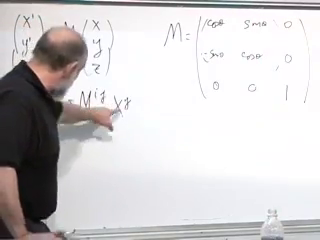
\includegraphics[width=0.82\textwidth]{lecture_05_figure_03.png}
\caption{공간 회전을 행렬 방정식과 첨자 표기법으로 각각 나타냈다.}
\lectureframe{01:00:40}
\end{figure}

\section{로런츠 행렬과 합성 속도}

\(x\)을 따른 운동에 대해, \(c=1\) 단위에서 로런츠 변환은 다음과 같다.
\begin{align}
x'&=\gamma_v(x-vt), & y'&=y,\nonumber\\
z'&=z, & t'&=\gamma_v(t-vx),
\end{align}
여기서
\begin{equation}
\gamma_v=\frac{1}{\sqrt{1-v^2}}.
\end{equation}
성분 순서를 \((x,y,z,t)\)로 쓰면 다음과 같다.
\begin{equation}
\begin{pmatrix}x'\\y'\\z'\\t'\end{pmatrix}
=
\begin{pmatrix}
\gamma_v&0&0&-\gamma_vv\\
0&1&0&0\\
0&0&1&0\\
-\gamma_vv&0&0&\gamma_v
\end{pmatrix}
\begin{pmatrix}x\\y\\z\\t\end{pmatrix}.
\label{eq:l5-lorentz-matrix}
\end{equation}

\begin{figure}[H]
\centering
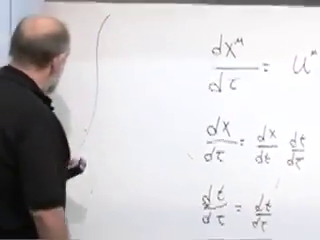
\includegraphics[width=0.82\textwidth]{lecture_05_figure_04.png}
\caption{로런츠 행렬. \(4\times4\) 성분 가운데 \(x\)와 \(t\) 성분만 서로 섞이고, \(y\)와 \(z\)는 변하지 않는다.}
\lectureframe{01:04:40}
\end{figure}

이제 행렬 곱셈으로 물리적 질문에 답해 보자. 한 관찰자가 우리에 대해 속도 \(v\)로 움직이고, 세 번째 관찰자가 그 관찰자에 대해 속도 \(u\)로 같은 축을 따라 움직인다고 하자. 뉴턴 역학에서는 \(w=u+v\)이 되어, 속도 \(3c/4\) 두 개가 합쳐져 \(3c/2\)가 될 수 있다. 상대론에서는 다른 법칙이 나와야 한다.

부스트에서 관련된 부분은 \(2\times2\) 행렬이다.
\begin{equation}
B(v)=\gamma_v
\begin{pmatrix}1&-v\\-v&1\end{pmatrix}.
\end{equation}
두 부스트를 합성하면
\begin{align}
B(u)B(v)
&=\gamma_u\gamma_v
\begin{pmatrix}1&-u\\-u&1\end{pmatrix}
\begin{pmatrix}1&-v\\-v&1\end{pmatrix}\nonumber\\
&=\gamma_u\gamma_v
\begin{pmatrix}
1+uv&-(u+v)\\
-(u+v)&1+uv
\end{pmatrix}.
\label{eq:l5-composed-boost}
\end{align}
비대각 성분과 대각 성분의 비로 결과 부스트의 속도를 구할 수 있다.
\begin{equation}
w=\frac{u+v}{1+uv}
\qquad(c=1).
\end{equation}
차원을 되살리면,
\begin{equation}
w=\frac{u+v}{1+uv/c^2}.
\label{eq:l5-velocity-addition}
\end{equation}

\begin{figure}[H]
\centering
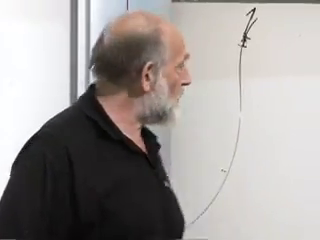
\includegraphics[width=0.82\textwidth]{lecture_05_figure_05.png}
\caption{부스트를 합성한 행렬과 자연 단위계에서의 속도 \(w=(u+v)/(1+uv)\).}
\lectureframe{01:15:35}
\end{figure}

\(u\)와 \(v\)가 각각 \(c\)에 가까우면 분자는 \(2c\)에 가까워지고 분모는 \(2\)에 가까워지므로, \(w\)는 \(2c\)가 아니라 \(c\)에 가까워진다. 더 일반적으로 식 ~\eqref{eq:l5-velocity-addition}은 광속보다 작은 입력 속도들을 광속보다 작은 결과 속도로 보낸다. 행렬 곱셈에 속도 제한이 자동으로 반영된 것이다.

\section{4-벡터와 보통 속도의 한계}

4-벡터란 네 성분이 시공간 좌표와 같은 방식으로 회전과 로런츠 부스트에 따라 변환하는 임의의 대상을 말한다. \(V^\mu\)가 4-벡터라면, 우리의 부호 관례에서
\begin{equation}
V_\mu=(-V^1,-V^2,-V^3,V^0),
\end{equation}
불변 노름은 다음과 같다.
\begin{equation}
V_\mu V^\mu=(V^0)^2-(V^1)^2-(V^2)^2-(V^3)^2.
\end{equation}
두 4-벡터 \(V^\mu\)와 \(W^\mu\)의 수축량
\begin{equation}
W_\mu V^\mu
=W^0V^0-W^1V^1-W^2V^2-W^3V^3
\end{equation}
도 마찬가지로 불변이다. 기준계에 따라 성분은 변하지만 수축량은 변하지 않는다.

보통 속도는 성분이 세 개뿐이다.
\begin{equation}
\mathbf v=\left(\frac{dx}{dt},\frac{dy}{dt},\frac{dz}{dt}\right).
\end{equation}
\(dt/dt=1\)를 덧붙여도 유용한 4-벡터가 되지는 않는다. 네 번째 성분은 자명하고, 이렇게 얻은 대상은 로런츠 변환 아래에서 선형적으로 변환하지 않는다. 좌표 시간 \(t\)은 기준계마다 달라지므로, \(t\)으로 미분하면 원하는 변환 법칙이 깨진다.

고유 시간을 쓰면 이 문제가 해결된다. 세계선을 따라 다음과 같이 정의하자.
\begin{equation}
u^\mu=\frac{dX^\mu}{d\tau}.
\label{eq:l5-four-velocity}
\end{equation}
미소량 \(dX^\mu\)는 4-벡터이고 \(d\tau\)는 불변이므로, 이 둘의 비는 4-벡터다. ``고유''라는 말은 분모에 있는 시계를 가리킨다.

연쇄 법칙으로 이 대상을 보통 속도와 관련지을 수 있다.
\begin{equation}
\frac{dx}{d\tau}=\frac{dx}{dt}\frac{dt}{d\tau},
\end{equation}
\(y\)와 \(z\)에 대해서도 마찬가지다. 식 ~\eqref{eq:l5-proper-time}에서
\begin{align}
\left(\frac{d\tau}{dt}\right)^2
&=1-\left(\frac{dx}{dt}\right)^2
    -\left(\frac{dy}{dt}\right)^2
    -\left(\frac{dz}{dt}\right)^2\nonumber\\
&=1-v^2
\qquad(c=1),
\end{align}
따라서
\begin{equation}
\frac{dt}{d\tau}=\gamma_v=\frac{1}{\sqrt{1-v^2}}.
\end{equation}
네 성분은 다음과 같다.
\begin{equation}
u^i=\gamma_v v^i,
\qquad
u^0=\gamma_v
\qquad(c=1).
\label{eq:l5-four-velocity-components}
\end{equation}
속도가 낮으면 \(u^i\simeq v^i\)이고 \(u^0\simeq1\)이다. 빛의 속도에 가까워지면 \(\gamma_v\)는 한없이 커지고 고유 속도는 보통 속도와 크게 달라진다.

\begin{figure}[H]
\centering
\includegraphics[width=0.82\textwidth]{lecture_05_figure_06.png}
\caption{고유 속도의 네 성분을 보통 속도와 로런츠 인자로 나타냈다.}
\lectureframe{01:34:40}
\end{figure}

보통 단위를 되살리고 \(X^0=ct\)를 사용하면, 여기서 쓰는 공간 성분 우선 순서에 따른 표준형은 다음과 같다.
\begin{equation}
U^\mu=(\gamma_v\mathbf v,\gamma_v c)
\end{equation}
불변 노름은
\begin{equation}
U_\mu U^\mu=c^2.
\end{equation}
따라서 모든 질량을 가진 입자는 공간 속도가 기준계에 따라 달라지더라도 크기가 같은 불변 노름의 4-속도를 갖는다.

\section{세계선의 접선}

식 ~\eqref{eq:l5-four-velocity}을 이해하는 데 익숙한 유클리드 공간의 예를 들 수 있다. 보통의 3차원 공간에서 곡선을 따라가면,
\begin{equation}
ds^2=dx^2+dy^2+dz^2.
\end{equation}
미소 변위 \((dx,dy,dz)\)는 곡선을 따라 향하지만 단위 벡터는 아니다. 이를 호의 길이로 나누면
\begin{equation}
\mathbf T=
\left(\frac{dx}{ds},\frac{dy}{ds},\frac{dz}{ds}\right),
\qquad
\mathbf T\cdot\mathbf T=1.
\end{equation}
상대론적 구성도 같은 생각을 따른다. 다만 유클리드 호의 길이 대신 고유 시간을 쓴다. 벡터 \(u^\mu=dX^\mu/d\tau\)는 세계선의 접선이다.

\begin{figure}[H]
\centering
\includegraphics[width=0.82\textwidth]{lecture_05_figure_07.png}
\caption{유클리드 공간에서 접선 벡터를 만드는 과정. 미소 변위 벡터를 호의 길이 요소 \(ds\)로 나눈다. 시간꼴 세계선을 따라서는 고유 시간이 이에 상응하는 역할을 한다.}
\lectureframe{01:39:30}
\end{figure}

\begin{classroomqa}
\audiencequestion{\(c=1\)라면 고유 시간과 고유 거리는 같은 건가요?}
\lecturerresponse{\(c=1\)로 두면 시간과 거리를 같은 단위로 나타낼 수 있지만, 시공간 기하학의 마이너스 부호가 사라지는 것은 아니다. 유클리드 유추에서 \(s\)은 공간 곡선을 따라 잰 보통 거리다. 시간꼴 세계선에서 \(\tau\)은 시계가 측정한 경과 시간이다. 구성은 서로 유사하지만 기하학은 다르다.}
\end{classroomqa}

한 번 더 미분하면 고유 가속도가 정의된다.
\begin{equation}
a^\mu=\frac{du^\mu}{d\tau}.
\end{equation}
뉴턴의 제2법칙을 상대론적으로 일반화할 때 \(d^2\mathbf x/dt^2\) 대신 써야 하는 물리량이 바로 이것이다. \(u_\mu u^\mu\)가 상수이므로,
\begin{equation}
\frac{d}{d\tau}(u_\mu u^\mu)=2u_\mu a^\mu=0,
\end{equation}
따라서 4-가속도는 민코프스키 내적에서 4-속도와 직교한다.\editorialnote{직교성은 불변 노름에서 바로 따라 나오며, 정의에서 얻는 다음 수학적 귀결로 여기에 덧붙였다.}

\section{4-운동량과 에너지}

운동량은 충돌과 붕괴에서 보존되므로 마지막 예로 살펴보자. 입자는 고정된 고유 질량 \(m\)을 가지며, 이를 정지 질량이라고도 한다. 이 질량은 속도에 따라 변하지 않는다. 상대론적 운동량은 이 고정된 질량과 4-속도의 곱이다.
\begin{equation}
p^\mu=mu^\mu.
\label{eq:l5-four-momentum}
\end{equation}
\(c=1\) 단위에서는,
\begin{equation}
p^i=\gamma_v m v^i,
\qquad
p^0=\gamma_v m.
\end{equation}
속도가 낮아 \(\gamma_v\simeq1\)이면 공간 성분은 뉴턴 역학의 운동량 \(m\mathbf v\)로 줄어든다. 고속에서는 이 성분들이 \(m\mathbf v\)보다 더 빠르게 커진다.

시간 성분은 에너지다. 보통 단위를 쓰고 \(X^0=ct\)로 두면,
\begin{equation}
P^\mu=(\mathbf p,E/c)
=(\gamma_v m\mathbf v,\gamma_v mc),
\end{equation}
따라서
\begin{equation}
E=\gamma_v mc^2
=mc^2\left(1-\frac{v^2}{c^2}\right)^{-1/2}.
\label{eq:l5-relativistic-energy}
\end{equation}

보통 역학을 되찾으려면 다음과 같이 두자.
\(\epsilon=v^2/c^2\ll1\). 이항 전개를 하면
\begin{equation}
(1-\epsilon)^p=1-p\epsilon+O(\epsilon^2).
\end{equation}
\(p=-1/2\)로 두면,
\begin{align}
E
&=mc^2\left(1-\frac{v^2}{c^2}\right)^{-1/2}\nonumber\\
&=mc^2\left[1+\frac12\frac{v^2}{c^2}
  +O\!\left(\frac{v^4}{c^4}\right)\right]\nonumber\\
&=mc^2+\frac12mv^2+O\!\left(\frac{mv^4}{c^2}\right).
\label{eq:l5-energy-expansion}
\end{align}

\begin{figure}[H]
\centering
\includegraphics[width=0.82\textwidth]{lecture_05_figure_08.png}
\caption{저속에서의 상대론적 에너지 전개. 정지 에너지와 뉴턴 역학의 운동 에너지가 드러난다.}
\lectureframe{01:51:30}
\end{figure}

첫째 항인 \(mc^2\)은 정지해 있을 때도 존재한다. 입자 집합과 각 입자의 질량이 변하지 않는 뉴턴 역학 문제에서는 그 항이 운동 전후에 같은 상수를 더하므로, 익숙한 장부 계산에서는 \(\tfrac12mv^2\)만 고려한다. 상대론에 따르면 버려진 그 상수도 처음부터 물리적인 에너지였다.

따라서 에너지와 운동량은 서로 무관한 보존 법칙이 아니다. 이들은 하나의 보존 벡터를 이루는 네 성분이다. 로런츠 부스트는 이들을 서로 섞는다. 한 관찰자가 에너지라고 부르는 것의 일부는 다른 관찰자에게 운동량으로 기여하며, 그 반대도 마찬가지다. 그렇더라도 고립계의 전체 4-운동량은 모든 관성계에서 충돌이나 붕괴 전후로 같다.

이 지점에서 상대론적 역학의 문턱에 이른다. 다음으로 할 일은 고유 가속도로 힘을 표현하고, 상대론적 파동 방정식, 특히 전자기와 빛을 지배하는 방정식을 이해하는 것이다.
